\documentclass[12pt, oneside]{report}
\usepackage[
backend=bibtex8,
style=ieee,
citestyle=numeric
] {biblatex}
\usepackage[top=2in,bottom=1in,right=1in,left=1in]{geometry}
\usepackage[document]{ragged2e}
\usepackage{setspace}
\usepackage{titlesec} % for formatting the chapter titles
\usepackage{graphicx}
\usepackage[titletoc,title]{appendix}
\usepackage{wrapfig}
\usepackage[font=small]{caption, subcaption}
\usepackage{hyperref}
\usepackage[table,xcdraw]{xcolor}

% Font packages and settings
\usepackage{fontspec}

\titleformat{\chapter}[block]
{\normalfont\huge\bfseries}{\thechapter}{20pt}{}
\titlespacing*{\chapter}
{0pt}{20pt}{20pt}
\setcounter{tocdepth}{2}
\setcounter{secnumdepth}{2}
\setlength{\parindent}{1cm}
\setmainfont{Times New Roman}
\doublespacing
\addbibresource{citations.bib}

\begin{document}
	\thispagestyle{empty}
	\pagenumbering{roman}

	\begin{center}
		\singlespacing
		\vspace{4in}
		THESIS TITLE\\
		\vspace{1in}
		Jacob Timothy Hill\\
		\vspace{1in}
		A dissertation submitted to the faculty at the University of North Carolina at Chapel Hill in partial fulfillment of the requirements for the degree of Doctor of Philosophy in the School of Information and Library Science.\\
		\vspace{1in}
		Chapel Hill\\
		2020
		\vspace{1in}
	\end{center}
	\begin{raggedleft}
		Approved By:\\
		Ryan Shaw\\
		Melanie Feinberg\\
		Jaime Arguello\\
		Omid Ghaemmagami\\
		Ted Underwood\\
	\end{raggedleft}
\newpage
\begin{center}
	\vspace*{\fill}
	\copyright 2020\\
	Jacob Timothy Hill\\
	ALL RIGHTS RESERVED
	\vspace{1in}
\end{center}
\newgeometry{top=2in,bottom=1in,right=1in,left=1in}
\begin{center}
	\textbf{ABSTRACT}
\end{center}
\newgeometry{margin=1in}
\setlength{\parindent}{15pt}
\tableofcontents
\newpage
\listoffigures
\chapter{Introduction}
\pagenumbering{arabic}
Overall argument: We are applying algorithms developed for information science and computer science tasks to humanities tasks and this is problematic because it requires significantly more interogation of the process, the bias in the data (text encoding, archival bias e.g. whats included and not included, etc.).

When moving into a new field like Digital Humanities it is important to explore some questions related to methodological fit. These explorations have to be done for different fields and different problems. We can't have one solution for all humanities probelms. The kind of work done thus far relates to some basic explorations of the application of algorithms to humanities problems, often without a clear idea of how to interpret the results, as well as some NLP work that addresses issues related to Arabic and Persian corpora. Before applying NLP problems to Bahá'í texts it is important to contextualize the probelms which entails framing them in such a way that computer scientists and humanists, to adopt an overly simplistic schema of the audienc, can engage in a common conversation.
\chapter{Literature Review}

\chapter{The Linguistic Setting}
\par

\par
The Bah\'{a}'\'{i} writings are something of a linguistic anomaly.
\par
Few writers have such a wide ranging audience in mind or adapt so much to the linguistic capacities/leanings of their audience.
\section{The ``Raw'' Data}
\par
The sample of Bah\'{a}'\'{i}  writings used in this study consists of nearly everything available on the authorized website of the Universal House of Justice (www.reference.bahai.org)–the elected governing body of the international  Bah\'{a}'\'{i} community–with the exception of some early scholarly attempts to compile the Bah\'{a}'\'{i} writings, such as those of `Abdu'l-Ham\'{i}d Ishr\'{a}q-Kh\'{a}vari, and a few largely derivative compilations. Including the former would require significant manual labor to separate the words of the author from the passages of Bah\'{a}'\'{i} scripture he compiles. Including the latter would add duplicate text, possibly skewing the results of the study through the multiplication of commonly occurring passages. Volumes consisting of scanned images without machine readable text were naturally excluded because of the significant work required to prepare them for computation. For a list of all published volumes included in the present study see \nameref{app-1}. For a relational view of the number of works in the sample compared to all extant works see \autoref{fig:works-table}.
\begin{figure}[htb]
\centering
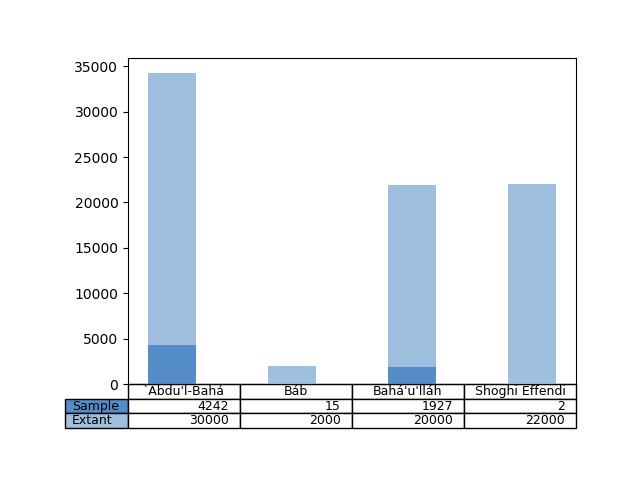
\includegraphics[width=15cm]{figures/works-table.png}
\caption[Bah\'{a}'\'{i} works sampled relative to all extant works]{Bah\'{a}'\'{i} works sampled relative to all extant works}
\label{fig:works-table}
\end{figure}
\par
The individual Bah\'{a}'\'{i} works were parsed from the published volumes listed in \nameref{app-1} and labelled with author and language (Arabic or Persian). This binary linguistic labelling at the level of the work may be somewhat misleading given the fluidity of language that is charicteristic of the Bah\`{a}'\'{i} writings. A more granular labelling strategy-say at the level of the sentence or paragraph-though ideal, would require an exponential increase in manual labor. By way of compromise, the works labelled `Arabic' are fully Arabic. The occasional Persian word, or Persianized Arabic word, may slip in but the general structure is Arabic. There are no Persian sentences, prepositions, or pronouns. Works were labelled manually, checked computationally, reinspected and relabelled if necessary. The checking step consisted of generating a list of high frequency Persian words, which included all prepositions and pronouns, and iteratively searching each Arabic text for words in this list. If the Arabic text contained any of the high frequency Persian words, it was reinspected and, if necessary, relabelled.
\par
This labelling strategy is justified by historical and cultural precedent. Persians, being largely Muslim, were expected to have some knowledge of the Arabic language–the language of the Qur'\'{a}n. Arab Muslims, on the other hand, were not expected to learn Persian. The impact of this cultural and historical phenomenon on the Bah\'{a}'\'{i} corpus is discernible in the larger number of wholly Arabic works–particularly among earlier among the earlier authors–as well as the frequency of lengthy Arabic passages in most Persian works. There are a significant number of Persian works without Arabic passages, but given the expectation that Persian readers would know some Arabic, the appearance of large segments of Arabic text in Persian works is commonplace.
\par
The implications of such a strategy are that the total number of Arabic and Persian words are skewed towards Persian (there are 706,426 Arabic words compared to 1,906,607 Persian). Most of the ``Persian'' works contain large sections of Arabic text which gets counted in the Persian word count. This, unfortunately, is unavoidable given that a more granular labelling approach is not presently feasible.
\par
In order to provide context, a large corpus of contemporary texts were selected for comparison, which included a collection of over 60,000 Persian poems (``and a few prose texts'') prepared by the Persian Digital Library Pilot Project (PDL) \cite{noauthor_persian_nodate} and nearly 350 lengthy Arabic works from the `Knowledge, Information Technology and the Arabic Book' (KITAB) \cite{maxim_romanov_openiti:_2019}. The selections from the KITAB project were limited to works from the 12th-14th centuries AH (October 26, 1688-November 21, 1979) which is roughly contemporaneous with the Bah\'{a}'\'{i} works sampled. All works in the PDL corpus were added without exception while works in the KITAB corpus that contained Persian passages were removed to maintain consistency with the linguistic labelling strategy applied to the Bah\'{a}'\'{i} corpus.
\section{Character Normalization}
\par
All computational linguistic work requires some level of pre-processing. There are several considerations that are peculiar to languages written in a modified form of the Arabic script. One such problem is the existence of ambiguous characters-characters with the same form, but different encodings \cite{jaf_semi-automatic_2016}. These characters appear the same to the human eye but have different underlying encodings. What appears to be the same letter in Persian and Arabic–the letter k\`{a}f for example–may in fact be two distinct encodings. Failure to conflate ambiguous characters results in the proliferation of vocabulary; a significant number of words that appear the same to the reader and were intended to be the same by the writer are treated as different words by the computer. Failure to remediate this issue prior to any down stream tasks can have significant negative effects on the outcome of those tasks. \begin{wrapfigure}{r}{.5\textwidth}
	\begin{minipage}{\linewidth}
		\centering\captionsetup[subfigure]{justification=centering}
		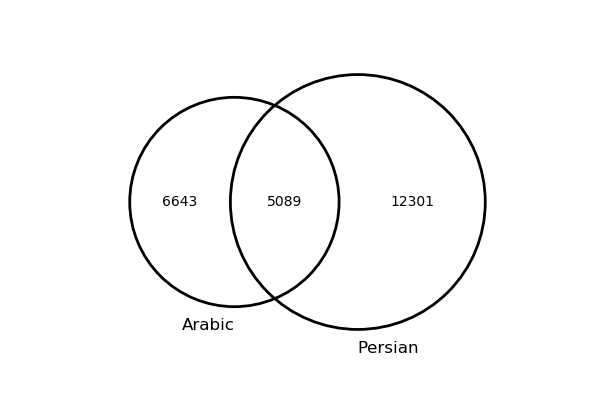
\includegraphics[width=\linewidth]{figures/venn-proc-one-freq5.png}
		\subcaption{}
		\label{fig:char-norm-a}\par\vfill
		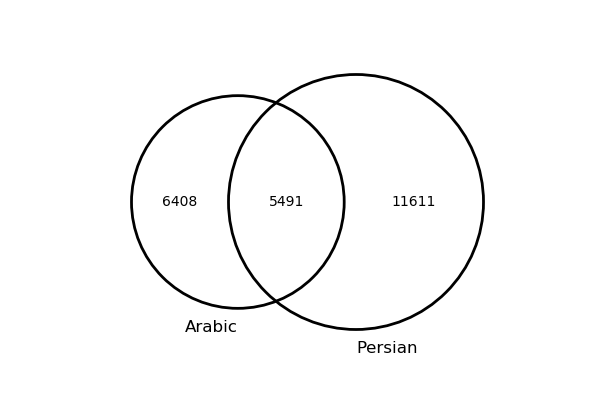
\includegraphics[width=\linewidth]{figures/venn-proc-two-freq5.png}
		\subcaption{}
		\label{fig:char-norm-b}
		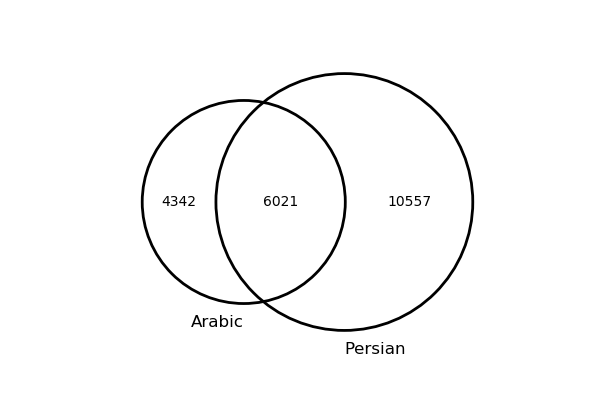
\includegraphics[width=\linewidth]{figures/venn-proc-three-freq5.png}
		\subcaption{}
		\label{fig:char-norm-c}
	\end{minipage}
	\caption[Venn diagrams depicting the effects of various processing decisions]{Arabic and Persian vocabulary with various levels of processing}\label{fig:char-norm}
\end{wrapfigure}These effects can be especially consequential if the object of interest is the interactions across language as the shared vocabulary–the loan words shared between languages that evince centuries of linguisitc and cultural exchange–are oblitered by the isolated processes through which the languages were encoded.
\par
Another issue affecting languages written in Arabic script is the inconsistent use of diacritical marks. In Arabic and Persian short vowels were historically not written, though they are
pronounced in speech. The reader is expected to know when to add the vowels, and which ones to add. There are, of course, a signigicant number of homographs which led to the subsequent development of diacritical marks that could be optionally added above or below letters to specify the following short vowel and thereby remove any ambiguity. Adoption has not been consistent, however, which compounds the vocabulary proliferation problem described above.
\par
A number of steps were taken to remediate this issue, the effects of which are summarized in
\autoref{fig:char-norm}. For all steps, the minimum frequency threshold was set at 5; words that occur less than five times across the whole corpus were removed. Diagram (a) shows the respective vocabulary with no data cleaning. Diagram (b) shows results after several language-agnostic cleanup steps were taken. Punctuation marks were removed as well as characters that produce only visual effects, such as spaces, tabs, and newline characters. Diagram (c) shows the results of removing character disambiguation and diacritical marks in addition to the steps taken in (b).
\par
The term ``pre-processing'', commonly used to describe this kind of work gives some indication of the level of importance it is given in the literature. Though it is deemed essential to any downstream task, in most computational linguistic research it is briefly described, or not at all. The field trends towards standardizing these practices and moving on to other, more interesting, things. Precedent often trumps rationale in determining which data cleaning steps are taken, and with good reason. Precedent has worked fine for decades and the circumstances have not changed. The application of computational linguistics strategies to humanities problems-problems they were not overtly designed to solve–warrants a re-examination and justification of these steps, as does the application to non-western languages. Both of these contextual changes introduce opportunities for confusion.
\par
The Venn diagrams in \autoref{fig:char-norm} provide insight into the effects pre-processing decisions can have. As is expected, without any intervention (a) there is a significant overlap in vocabulary. After all, many of the Persian texts contain Arabic passages and Persian, in general, is riddled with Arabic vocabulary. Language agnostic processing steps reduced the total vocabulary by 2.2\% (523 words), the Arabic vocabulary by 3.5\% (235 words), and the Persian vocabulary by 5.6\% (690 words), while the intersection increased by 7.9\% (402 words). Removing diacritical marks and conflating ambiguous characters reduced the total vocabulary by an additional 11\% (2,590 words), the Arabic vocabulary by 32\% (2,066 words), and the Persian vocabulary by 9.1\% (1,045 words), while increasing the intersecting vocabulary by 9.7\% (530 words). The reduction in vocabulary consisted exclusively of non-existent words–side effects of the text encoding process or typographical errors.
\par
It is worth noting, also, the effect the minimum frequency threshold has on vocabulary. One of the of implications of Zipf's law on natural language is the common existence of a long tail of words that occur only once, or a few times. Removing these words helps to speed up computation and reduce noise; words that occur only once can have no interaction effects and words that occur only a few times do not provide enough data to draw statistically significant conclusions. With no pre-processing 243,639 words were removed, with language agnostic pre-processing only 163,692 words were removed, and with language agnostic processing, removal of diacritical marks and conflation of ambiguous characters only 103,824 words were removed. The trend towards discarding fewer words with each step of proceseeing is a clear indication of the efficacy of these techniques; nearly 140,000 words were sparred from removal. The raw count is not an adequate appraisal of the value of these techniques, however. Bearing in mind the objective of representing this vocabulary as a single matrix, these ~140,000 words take on added significance.
\par
To illustrate this point and simultaneously delineate the limitations of the adopted strategies consider the word `kalima`, an Arabic loan word meanings `word`. The first letter `kaf` has a different encoding in Arabic and Persian systems. Given that text encoding is not well understood by your average typist and considering that many of these typists may know Arabic and Persian and use both keyboards the word will bifurcate in both languages resulting in two forms in each langauge. The word `kalima` has a further problem with its final letter. In the Arabic original form it ends in ta marbuta, a letter indicating the feminine gender of the word. This letter is not found in Persian and is replaced by the letter `heh`, a somewhat similar looking letter that also exisits in Arabic. Adding in this results in for different possible forms for the same word–Arabic kaf... ta marbuta (form 1), Persian kaf... heh (form 2), Arabic kaf... heh (form 3), Persian kaf... ta marbuta (form 4). Normalizing the kaf would eliminate forms 2 and 4. For many words that completely remove the problematic effects of divergent text encodings. Unfortunately there is no easy solution for the heh ending adopted in Persian. Since it is used in Arabic, and often at the end of words, it cannot be blindly replaced with a ta marbuta. This would fix words like kalima while creating significant noise in the process. Normalizing variant text encodings is only a solution for vocabulary proliferation problems resulting from the historical circumstances of text encoding in Arabic and Persian. It cannot solve problems resulting from other historical processes.
\par
Failure to adequately prepare language data for down stream tasks delegitimizes the outcomes of those tasks. Meaningless sequences of encodings will erroneously be treated as words and examined for statistical significance while meaningful words will be discarded. This point is well established. What is less not well acknowledged, the importance of which is likely completely lost on many digital humanitsts, is the need for local processing models. Global language models-one size fits all approaches-can be problematic in unexpected ways. Languages have developed through unique historical and cultural circumstances. Failure to adequately understand and respond to the historical processes in which the language developed and was encoded for computational processing can undermine the whole process.
\section{A Range of Linguistic Modes}
\par
The Bah\'{a}'\'{i} writings in general, and the writings of Bah\'{a}'u'llah in particular, are comprised of numerous styles or genres. Bah\'{a}'u'llah demonstrates an unusual, perhaps unique, ability to adjust the style of His writing to a multitude of ends.
In a setting in which religion and culture appeared as fixed mountains, He showed an uncanny ability to sweep them aside, in favor of an ever more embracing vision.
In the religious and cultural diversity of His audience, in His demonstrated ability to write in a manner approachable to that audience, in His ability to transcend fixed literary genres, in the range of His vocabulary and grammatical prowess-in all these Bah\'{a}'u'llah shows a remarkable awareness of contemporary cultural, religious, and linguistic norms and a desire to transcend them in favor of ever wider horizons.
\par
In the Suratu'l-Haykal, Bah\'{a}'u'llah wrote ``We have revealed Our verses in nine different modes... Should it be Our wish, We would reveal them in countless other modes.''
A clear identification of these modes was never made by Bah\'{a}'u'llah or either of His authorized interpreters and it is likely that He did not wish His audience to become overly fixated on such a classification schema.
Evidence of Bah\'{a}'u'llah's view towards such schemas can be found in works such as 'The Seven Valleys' and 'The Gems of Divine Mysteries'.
In the former He delineates a series of steps that a seeker must pass through in his quest for the Beloved.
In the latter the steps are reworked, and some of which are renamed.
In a later work He offers insight into His perspective on these stages and why they were adopted at all: ``This treatise [The Seven Valleys] was revealed in the language of the people, in the days prior to Our Declaration. The occasion for its revelation was the receipt of a letter addressed to the Most Holy Court in ‘Iráq from a man of Sunní persuasion, who was both a scholar and a mystic. This treatise was therefore revealed, in accordance with divine wisdom, in the manner that was current amongst the people. However, in this day, every soul who hath fixed his gaze upon the Supreme Horizon, and hath recognized the one true God, hath verily attained unto every one of the seven valleys or seven stations mentioned therein \cite{}.''
In several other works Bah\'{a}'u'llah advances other schemes with different stages.
These schemas are irreconcilable in some cases indicating His frequent willingness to respond from the framework of His audience and gradually rework that framework, discarding concepts that served as obstacles to the unification of humanity, often accepting or ignoring harmless components of that framework, and recasting the remainder in a new form that redeployed existing literary tropes, tropes that could, to the inattentive reader, be mistaken for the substance of the framework.
\par
It is uncertain if Bah\'{a}'u'llah's linguistic modes should be viewed in the same light but the fact that He never endeavored to describe them in any detail suggests their relative importance in His overall message.
Nevertheless, others have attempted to delineate these modes.
Jin\'{a}b-i-F\'{a}dil-i-M\'{a}zindar\'{a}n\'{i}, a prominent early scholar of the Bah\'{a}'\'{i} Faith, made a preliminary classification which attempted to identify these nine modes as: those tablets with the tone of authority, those with the tone of servitude, those interpreting past scripture, those specifying of laws and ordinances, mystical writings, writings about government and world order, writings about the various branches of learning, writings calling for education, good character and virtues, and works treating social teachings \cite{}.
It is worth noting that M\'{a}zindar\'{a}n\'{i}'s schema constitutes a significant departure from B\'{a}b\'{i} and Islamic discourse. The Arabic term \underline{sh}a'n, meaning mode or style, can be found in the writings of the B\'{a}b and, more generally, in Islamic thought.
Nader Saiedi points out that there were four modes in Islam: divine verses; prayers and supplications; commentaries and sermons; and rational, educational, and philosophical discourse \cite{saiedi_gate_2008}.
To these four modes, the B\'{a}b added the Persian mode-the idea that God would speak in a language other than Arabic being quite revolutionary-which comprised the other four.
\par
The four modes of Islam roughly correlate with the perspective of the speaker.
The first mode (divine verses) represents the voice of God speaking directly to His creation.
The second mode (prayers and supplications) is the voice of creation responding to its Creator.
Together the two modes constitute a dialogue between the Creator and the creation.
Linguistically, they might be distinguished by the prominence of first and second person pronouns and verbs conjugated in the first and second person.
See, for example, the two following passages, the first of which is in the mode of divine verses and the second in the mode of supplication and prayer: ``O SON OF MAN! \emph{I loved thy} creation, hence \emph{I created thee}. Wherefore, do \emph{thou love Me}, that \emph{I} may \emph{name thy} name and \emph{fill thy} soul with the spirit of life \cite{bahaullah_hidden_2002}.'' ``Glory be to \emph{Thee}, O \emph{my} God!  \emph{Thou hearest Thine} ardent lovers lamenting in their separation from \emph{Thee}, and such as have recognized \emph{Thee} wailing because of their remoteness from \emph{Thy} presence \cite{}.''
The third (commentaries and sermons) and fourth modes (rational, educational, and philosophical discourse) would be characterized by a predominance of third person pronouns and verbs as the subject matter is further removed from the speaker.
Thus the four modes correspond to varying degrees of remoteness from the Divine creator and are affirmed, respectively, by the verses ``I am God'', ``Thou art God'', ``He is God'', and ''He is God Who is'' \cite{saiedi_gate_2008}.
To these modes, the B\'{a}b added the Persian mode, the content of which could be any of the other four modes \cite{saiedi_gate_2008} and would have the same linguistic markers to the extent that these markers are shared between the Arabic and Persian languages.
\par
It is clear that many of Bah\'{a}'u'llah's readers would have been familiar with this discourse and His statement regarding the revelation of His verses in ``nine modes`` would have conjured up this discourse in their minds.
The first three categories in M\'{a}zindar\'{a}n\'{i}'s classification overlap with those established in Islamic thought and reaffirmed by the B\'{a}b.
Categories four through nine depart from the established norm in favor of a subject oriented schema.
Moreover, many of M\'{a}zindar\'{a}n\'{i}'s later categories are not unique to the writings of Bah\'{a}'u'llah; they can be found in Islamic and B\'{a}b\'{i} scripture as well.
In 'The Epistle to the Son of the Wolf', Bah\'{a}'u'llah's last major work, He writes: “At one time We spoke in the language of the lawgiver; at another in that of the truth-seeker and the mystic \cite{}”.
It is possible that M\'{a}zindar\'{a}n\'{i} viewed this statement in light of these linguistic modes since these correspond with two of the modes he identified, but I see no clear reason to conflate the two.
Religious law and the mystic search for the Beloved are often juxtaposed in Islamic discourse and Bah\'{a}'u'llah addresses them together in many prior works.
M\'{a}zindar\'{a}n\'{i}'s shift to subject as the organizing principle of Bah\'{a}'u'llah's literary modes constitutes a departure from Islamic and B\'{a}b\'{i} discourse and, in my mind, is in need of further justification.
\par
The point of such a departure is to demonstrate Bah\'{a}'u'llah's intentionality in writing in many different styles even if He never intended to, or we cannot concretely, crystallize His stylistic schema into discrete genres.
Such a point is important given that the variety of styles-whether style is operationalized as subject matter, perspective, or something else entirely-are likely to carry linguistic traces that are discernible through computational processes and may have implications for the choice of algorithms and the interpretation of their outputs.
\begin{table}[]
	\centering
	\begin{tabular}{|l|l|r|r|}
		\hline
		\rowcolor[HTML]{EFEFEF}
		\textbf{} & \textbf{File Path}                       & \textbf{Word Count}         & \textbf{Percent Persian}      \\ \hline
		1         & bahaullah/text/bahaullah-amtm-21-fa.txt  & \cellcolor[HTML]{FFFFFF}323 & \cellcolor[HTML]{FFFFFF}79.88 \\ \hline
		\rowcolor[HTML]{EFEFEF}
		2         & bahaullah/text/bahaullah-amtm-22-fa.txt  & 255                         & 91                            \\ \hline
		\rowcolor[HTML]{FFFFFF}
		3         & bahaullah/text/bahaullah-amtm-23-fa.txt  & 182                         & 91.76                         \\ \hline
		\rowcolor[HTML]{EFEFEF}
		4         & bahaullah/text/bahaullah-amtm-24-fa.txt  & 187                         & 76.5                          \\ \hline
		\rowcolor[HTML]{FFFFFF}
		5         & bahaullah/text/bahaullah-amtm-25-fa.txt  & 522                         & 82.76                         \\ \hline
		\rowcolor[HTML]{EFEFEF}
		6         & bahaullah/text/bahaullah-amtm-37-fa.txt  & 252                         & 71.43                         \\ \hline
		\rowcolor[HTML]{FFFFFF}
		7         & bahaullah/text/bahaullah-aqa2-70-fa.txt  & 1292                        & 78.49                         \\ \hline
		\rowcolor[HTML]{EFEFEF}
		8         & bahaullah/text/bahaullah-st-004-fa.txt   & 130                         & 86.15                         \\ \hline
		\rowcolor[HTML]{FFFFFF}
		9         & bahaullah/text/bahaullah-st-058-2-fa.txt & 206                         & 72.82                         \\ \hline
		\rowcolor[HTML]{EFEFEF}
		10        & bahaullah/text/bahaullah-st-098-fa.txt   & 165                         & 72.12                         \\ \hline
		\rowcolor[HTML]{FFFFFF}
		11        & bahaullah/text/bahaullah-st-199-fa.txt   & 45                          & 75.6                          \\ \hline
	\end{tabular}
	\caption{Works of Bah\'{a}'u'llah possibly written in a pure Persian }
	\label{tab:pure-persian}
\end{table}
\par
Evidence of Bah\'{a}'u'llah's linguistic capacity can be found in the range of the vocabulary He uses in different works. The spectrum ranges from pure Persian works-those with no Arabic vocabulary-to pure Arabic works and everything in between. There was a movement contemporary to Bah\'{a}'u'llah, and still in existence today, that aimed to cleanse the Persian language of all of its acquired Arabic baggage. Bah\'{a}'u'llah was not an advocate of this movement. In a moment of unusual candor He asserted: ``There are many things which have not been expressed in Persian, that is to say, words referring to such things have not been devised, whilst in Arabic there are several words describing the same thing. Indeed there existeth no language in the world as vast and comprehensive as Arabic \cite{bahaullah_tabernacle_2006}.'' Yet, at times He deferred to the wonts of His correspondents and demonstrated His capacity to write in pure Persian. A query for works largely situated in the Persian sphere of the Venn diagram depicted in \autoref{fig:venn-pers} returns several works written in this style. If the cutoff level is set at 70\%, that is at least 70\% of the words present in the work are only present in other Persian works, 11 works are returned \ref{tab:pure-persian} which can roughly be clustered into three groups: false positives, intentionally pure Persian works, and works with relatively few Arabic words that are symptomatic of another cause.
\par
Numbers 6, 9 and 11 are likely false positives. The fact that they have relatively few Arabic words is likely attributable to something other the Bah\'{a}'u'llah's intention to write without the use of Arabic vocabulary. Work 11, for example, has only 45 words. The fact that such a small percentage of them are of Arabic origin is likely due to the sample size. Works 6 and 9 have a higher percentage of Arabic loan words than most of the works in this list and there seems to be no discernable pattern to their placement within the works.
\par
Works 1, 4, 7, 8, 10 all have relatively few Arabic loan words though this is likely attributable to other factors. Works 1 and 4 are published in consecutive order with other tablets addressed to believers of Zoroastrian background \cite{bahaullah_majmu`ih-i_1920}. The sparcity of Arabic vocabulary may stem from the Author's awareness of the cultural and linguistic background of His audience without the overt intention to avoid Arabic words altogether. Likewise, works 7, 8, and 10 share a genre. The are all poems reminiscent of the major Persian Sufi classical poets: 'Att\'{a}r, Sa'di, Rumi and H\'{a}fez. A predominate Persian vocabular sprickled with Arabic words is charachteristic of the genre.
\par
There seems to be more deliberateness to the avoidance of Arabic words in works 2, 3, and 5. They were published in consecutive order with works 1 and 4 and were likewise addressed to believers of Zoroastrian heritage. Works 1, 4, and 5 were later translated in a volume of other works addressed to early Zoroastrian converts to the Bah\'{a}'\'{i} Faith \cite{bahaullah_tabernacle_2006}. The introduction to the volume explicitly mentions that the recipient of work number 1, M\'{a}nik\underline{ch}\'{i} Ṣ\'{a}ḥib, requested that Bah\'{a}'u'llah respond–and write exclusively henceforth–in pure Persian. Bah\'{a}'u'llah acknowledged this request by penning His reply in pure Persian, save the 75 word closing section which is a mixture of Arabic and Persian. Work number 2 found 9\% of the words in the Arabic vocabulary but these words consist largely of homonyms such as the word `\underline{sh}ahr', which means `announcement' or `declaration' in Arabic and `city' in Persian. The other words are clearly of Persian origin; their inclusion in the intersection of the Venn diagram \autoref{fig:venn-pers} must be attributed to their appearnace in an Arabic work or, possibly, to a mislabelling of one or more files. Work number 3 is of the same type; all words except the word `ism' are of Persian origin.
\begin{wrapfigure}{r}{.5\textwidth}
	\centering\captionsetup[subfigure]{justification=centering}
	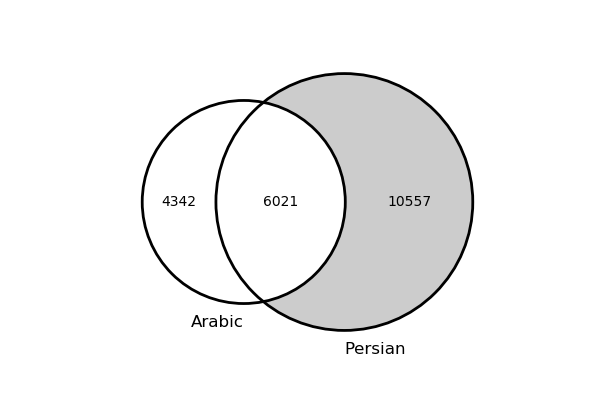
\includegraphics[width=\linewidth]{figures/venn-persian.png}
	\caption[Venn diagram with Persian section highlighted]{Pure Persian works can be identified by querying for works with vocabulary situated largely in the Persian section}\label{fig:venn-pers}
\end{wrapfigure}
\par
The examples above testify to Bah\'{a}'u'llah's ability to avoid words of Arabic origin altogether but they seem exceptional from a linguistic perspective. Generally His Persian writing is riddled with Arabic vocabulary. In many cases there are significanly more Arabic than Persian words. For example, in a letter to Zaynu'l-Muqarrab\'{i}n, nearly eighty percent of the words are of Arabic origin \cite{bahaullah_muntakhabati-az_163}. There are many other such examples. In these cases the Persian language is like the mortar hodling together the Arabic bricks; the verbs and some of the conjunctions are the only non-Arabic words in the text.
\par
The same search strategy cannot be employed for revealing pure Arabic works. The fact that Arabic words are commonplace in the Persian language implies that the vocabulary of many pure Arabic works would have one foot firmly in the intersection between the two languages. Roughly 60\% of the Arabic vocabulary also appears in Persian works whereas only 36\% of the Persian vocabulary is used in Arabic works. Given that the Persian words do not abound in the Arabic language, there are sufficient examples of Bah\'{a}'u'llah's Arabic with little to no Persian influence.
\par
The quality of Bah\'{a}'u'llah's writing in both Arabic and Persian is something of a controversy. On one hand His writings have won the praise of renowned experts such as Khalil Gibran, according to a the third hand account of Marzieh Gail, \cite{gail_world_1978} and Edward Granville Browne who wrote of the Kitab-i-Iqan: ``it is a work of great merit, vigorous in style, clear in argument, cogent in proof, and displaying no slight knowledge of the Bible, Qur'an, and Tradition'' \cite{momen_selections_1987}. On the other hand, He has ammassed a large number of critics. Such opinions-both positive and negative-are highly subjective and of little use in determining Bah\'{a}'u'llah's linguistic competence. There are better ways to document Bah\'{a}'u'llah's linguistic versatility and prowess.
\par
Style, or literary genre, is certainly a fluid category.  Assigning boundaries to genres can be problematic. Yet identifying stylistic similarities between groups of literary works can shed light on questions of influence and awareness. The range of styles found among Bah\'{a}'u'llah's extant writings is noteworthy in this respect. Frank Lewis lists at least six distinct styles exemplified in His writings: the tradition of rhymed prose (saj'); tafsir; the classical Persian Sufi literary tradition exemplified by 'Att\'{a}r, Sa'di, Rumi and H\'{a}fez; the b\'{a}z ga\underline{sh}t adab\'{i} style which began as a counter movement to the sabk-e\'{i} style; the gnomic tradition (andarz); and the Persian gnostic tradition \cite{lewis_frank_scripture_1997}. William McCants notes the Sh\'{i}'\'{i} narrative structure ``underlying most of His epistles and homilies \cite{mccants_wronged_2002}.'' With little effort exemplars of other literary genres could be found in His writings. However, those already listed are sufficient to demonstrate the point that a number of disparate styles are contained within the corpus of Bah\'{a}'u'llah's writings.
\par
An even more impressive example of Bah\'{a}'u'llah's command of Arabic and Persian and His ability to write with precision can be found in the Hidden Words \cite{bahaullah_hidden_2002}. At the time of the revelation of the Hidden Words (1857) Bahá'u'lláh's audience would have been divided into four exclusive groups: Sunni, Shi'i, Wujudies and Shuhudis. Each of these, in turn, would be divided into opposing factions: Akhbaris, Usulis, and Shaykhis \cite{lawson_todd_globalization_2005}.  Bah\'{a}'u'llah wrote the Hidden Words in such a way that it would appeal to each faction. Quotations are woven throughout in paraphrase, there is no mention of a proper name that could signal an allegiance to any faction, no isnads, no legalistic doctrines or cultic pronouncements \cite{lawson_todd_globalization_2005}. What remains is something that could be seen by all as pure religion. ``A religion apparently unencumbered by the tragedy of history, appearing as a restatement of basic truths through the medium of a compelling religious literary art in both languages of the city: Arabic (71 `verses' and Persian (82 `verses') \cite{lawson_todd_globalization_2005}.'' Such an accomplishment is extraordinary given the sectarian nature of the religious discourse of 19th century Baghdad. Moreover, it shows a profound awareness of the discourse of each faction; in order to know which words to avoid, Bah\'{a}'u'llah had to be aware of which were most strongly identified with each sect. The work suggests a clear intent to elevate the minds of His audieance beyond such sectarian discourse and serves as aprofound example of His command of both languages.
\section{Comparative Linguistics}
\par
Another way to explore the linguistic characteristics of Bah\'{a}'u'llah's writings is through comparision to other authors. There are a number of methods that have been used for this purpose, many of which cannot be applied to the writings of Bah\'{a}'u'llah. For example, Justin Rice uses avarage sentence length as a metric to distinguish the style of Hemmingway's writings from that of other writers \cite{justin_rice_what_2018}. In classical Arabic and Persian, and in the writings of Bah\'{a}'u'llah specificaly, the period is an afterthought. It is used inconsistently when it is used at all and it must, until proven otherwise for each text, be treated as what Gennete refers to a `paratextuality'–an element outside of the text that influences its reading \cite{genette_gerard_palimpsests:_1997}. Periods in English, and often in modern Arabic and Persian, are part of the author's literary production; they are added by the author and can be used as evidence of his or her writing style. In the writings of Bah\'{a}'u'llah periods were added by scribes or publishers, if at all, and cannot therefore be used as evidence of writing style. Without periods there is no reliable way of determining sentence length which makes this metric inappropriate for the task at hand. Other examples could be given but this should be sufficient to demonstrate that stylometric methods are context dependent; any given method cannot be assumed to hold accross language and time.
\par
Among the methods that can safely be used to compare the writings of Bah\'{a}'u'llah to contemporary authors are average word length \cite{justin_rice_what_2018}, lexical richness \cite{justin_rice_what_2018}, and the chi-squared statistic  \cite{kilgarriff_comparing_2001} \cite{laramee_introduction_2018}. Word length

\begin{figure}[htb]
	\centering
	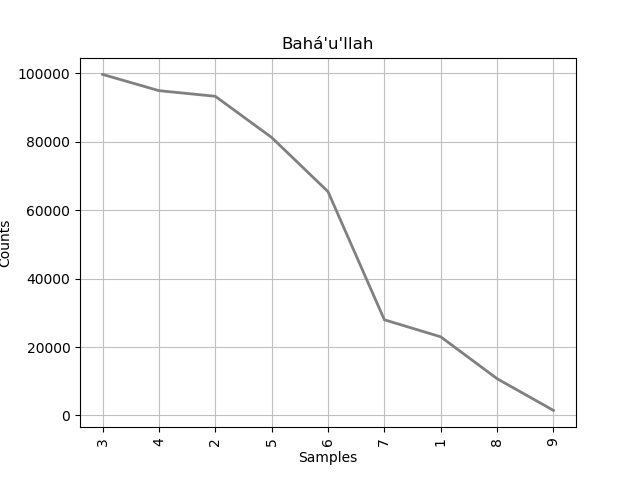
\includegraphics[width=15cm]{figures/word-length-bahaullah.png}
	\caption[Most common word lengths used by Bah\'{a}'u'llah]{Most common word lengths used by Bah\'{a}'u'llah}
	\label{fig:word-length-bahaullah}
\end{figure}
\begin{figure}[htb]
	\centering
	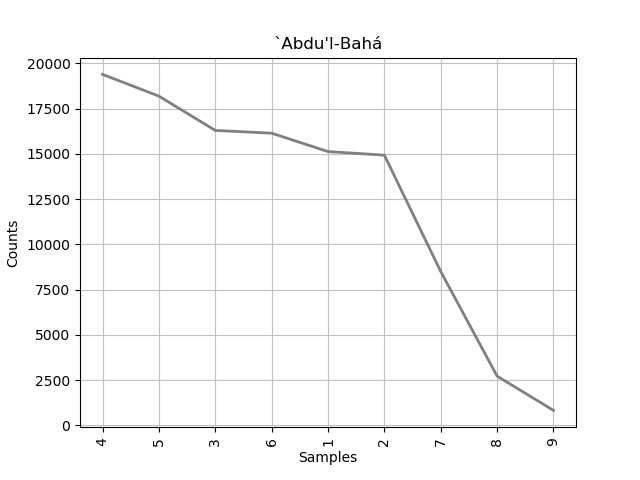
\includegraphics[width=15cm]{figures/word-length-abdulbaha.png}
	\caption[Most common word lengths used by `Abdu'l-Bah\'{a}]{Most common word lengths used by `Abdu'l-Bah\'{a}}
	\label{fig:word-length-abdulbaha}
\end{figure}
\begin{figure}[htb]
	\centering
	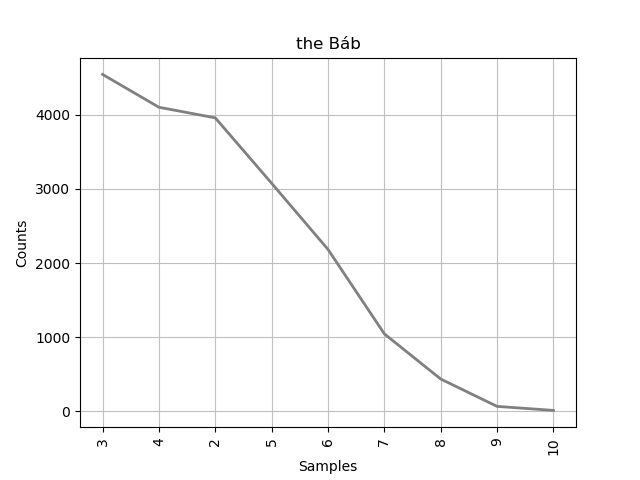
\includegraphics[width=15cm]{figures/word-length-bab.png}
	\caption[Most common word lengths used by the B\'{a}b]{Most common word lengths used by the B\'{a}b}
	\label{fig:word-length-bab}
\end{figure}
\begin{figure}[htb]
	\centering
	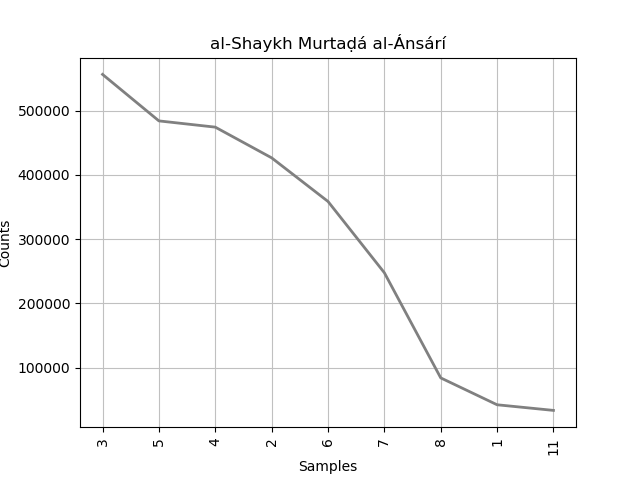
\includegraphics[width=15cm]{figures/word-length-shaykh-murtada.png}
	\caption[Most common word lengths used by al-Shaykh Murtaḍ\'{a} al-\'{A}ns\'{a}r\'{i}]{Most common word lengths used by al-Shaykh Murtaḍ\'{a} al-\'{A}ns\'{a}r\'{i}}
	\label{fig:word-length-murtada-ansari}
\end{figure}
\section{Conclusion}
Bah\'{a}'u'llah clearly adapted His writing style-genre, subject matter, and vocabulary-to His intended audience.

What you have is a highly deliberate collection of writings with ties to a plethora of genres and styles and yet linguistically distinct in many respects. That is, the position Bahá’u’lláh takes is both deliberately linked to past discourse and simultaneously	distinct.


\chapter{Word Embeddings}

\chapter{Conclusion}
\newpage
\begin{appendix}
\addcontentsline{toc}{chapter}{Appendices}
\chapter*{Appendix A: Bah\'{a}'\'{i} Published Volumes}
\addcontentsline{toc}{section}{Appendix A: Bah\'{a}'\'{i} Published Volumes}
\label{app-1}
\begin{table}[ht]
	\setlength{\tabcolsep}{18pt}
	\begin{tabular}{ll}
	\textbf{Author} & \textbf{Title} \\
		`Abdu'l-Bah\'{a}	& Majm\`{u}`eh Mon\`{a}jath\`{a} Ha\d{d}rat `Abdu'l-Bah\'{a} \\
	`Abdu'l-Bah\'{a}	& Makat\`{i}b Ha\d{d}rat `Abdu'l-Bah\'{a} Jild 1 \\
	`Abdu'l-Bah\'{a}	& Makat\`{i}b Ha\d{d}rat `Abdu'l-Bah\'{a} Jild 2 \\
	`Abdu'l-Bah\'{a}	& Makat\`{i}b Ha\d{d}rat `Abdu'l-Bah\'{a} Jild 3 \\
	`Abdu'l-Bah\'{a}	& Makat\`{i}b Ha\d{d}rat `Abdu'l-Bah\'{a} Jild 4 \\
	`Abdu'l-Bah\'{a}	& Makat\`{i}b Ha\d{d}rat `Abdu'l-Bah\'{a} Jild 5 \\
	`Abdu'l-Bah\'{a}	& Makat\`{i}b Ha\d{d}rat `Abdu'l-Bah\'{a} Jild 6 \\
	`Abdu'l-Bah\'{a}	& Makat\`{i}b Ha\d{d}rat `Abdu'l-Bah\'{a} Jild 7 \\
	`Abdu'l-Bah\'{a}	& Makat\`{i}b Ha\d{d}rat `Abdu'l-Bah\'{a} Jild 8 \\
	`Abdu'l-Bah\'{a}	&  Maq\`{a}leh Sha\underline{kh}si S\'{i}\'{a}\d{h} \\
	`Abdu'l-Bah\'{a}	&  Muf\'{a}wa\d{d}\'{a}t \\
	`Abdu'l-Bah\'{a}	& Munta\underline{kh}ib\'{a}ti az Makat\`{i}b Ha\d{d}rat `Abdu'l-Bah\'{a} Jild 1 \\
	`Abdu'l-Bah\'{a}	& Munta\underline{kh}ib\'{a}ti az Makat\`{i}b Ha\d{d}rat `Abdu'l-Bah\'{a} Jild 2 \\
	`Abdu'l-Bah\'{a}	& Munta\underline{kh}ib\'{a}ti az Makat\`{i}b Ha\d{d}rat `Abdu'l-Bah\'{a} Jild 3 \\
	`Abdu'l-Bah\'{a}	& Munta\underline{kh}ib\'{a}ti az Makat\`{i}b Ha\d{d}rat `Abdu'l-Bah\'{a} Jild 4 \\
	`Abdu'l-Bah\'{a}	& Munta\underline{kh}ib\'{a}ti az Makat\`{i}b Ha\d{d}rat `Abdu'l-Bah\'{a} Jild 5 \\
	`Abdu'l-Bah\'{a}	& Munta\underline{kh}ib\'{a}ti az Makat\`{i}b Ha\d{d}rat `Abdu'l-Bah\'{a} Jild 6 \\
	`Abdu'l-Bah\'{a}	& Ta\underline{dh}kirat al-Vaf\`{a}' \\
	B\'{a}b & Munta\underline{kh}ib\'{a}t \'{A}y\'{a}t az \'{A}th\'{a}r Ha\d{d}rat Nuq\d{t}eh Awl\`{a} \\
	Baha'u'll\'{a}h & Kit\`{a}b-i-\`{A}qdas \\
	Baha'u'll\'{a}h & Kit\`{a}b-i-\`{I}q\`{a}n \\
	Baha'u'll\'{a}h & Kalim\`{a}t Makn\`{u}neh F\`{a}rs\`{i} \\
	Baha'u'll\'{a}h & Kalim\`{a}t Makn\`{u}neh `Arab\`{i} \\
	Baha'u'll\'{a}h & Majm\`{u}`eh \`{A}lv\`{a}h b`ad az Kit\`{a}b-i-\`{A}qdas \\

	\end{tabular}
\end{table}
\end{appendix}
\singlespacing
\printbibliography
\end{document}
